\chapter{Risultati}
% Tabelle e grafici di ogni esperimento, con confronti fra i continual
\section{Risultati finali}
\paragraph{WESAD} Usando come modello due layer GRU da 18 unità, su WESAD ho ottenuto i seguenti risultati:

\begin{table}[h]
\footnotesize
    \begin{tabular}{l|c|c|c|c|c|c|c}
        \textbf{Scenario} & \textbf{Epoche} & \textbf{Tempo} & \textbf{Acc.} & \textbf{ACC} & \textbf{BWT} & \textbf{FWT} & \textbf{Memoria}\\
        \hline
        \textbf{Offline} & 28 & 94,69s & 99,07 & - & - & - & 2061,40 Mb\\
        \textbf{Continual} & 49,14$\pm$33,67 & 947,24s & 73,13$\pm$4,02 & 0,7721 & 0,0343 & 0,5397 & 2173 Mb\\
        \textbf{Cumulative} & 39,71$\pm$19,91 & 2786s & 81,97$\pm$8,67 & 0,961 & 0,1383 & 0,4674 & 2291,45 Mb\\
        \textbf{Replay} & 41,14$\pm$21,19 & 1063,51s & 78,29$\pm$3,32 & 0,7849 & -0,002 & 0,4582 & 2184,77 Mb\\
        \textbf{Episodic} & 35$\pm$26,26 & 1088,29s & 82,13$\pm$6,60 & 0,9095 & 0,0841 & 0,4226 & 2097,47 Mb\\
        \textbf{EWC} & 29,71$\pm$17,38 & 1342,81s & 70,74$\pm$4,74 & 0,7251 & 0,0113 & 0,4698 & 2187,40 Mb\\
        \textbf{LWF} & 44,29$\pm$18,30 & 3282,51s & 69,09$\pm$5,82 & 0,7419 & 0,0451 & 0,3248 & 2121,31 Mb\\
    \end{tabular}
    \caption{Risultati WESAD}
    \label{tab:reswesad}
\end{table}
\begin{figure}[h]
	\begin{center}
		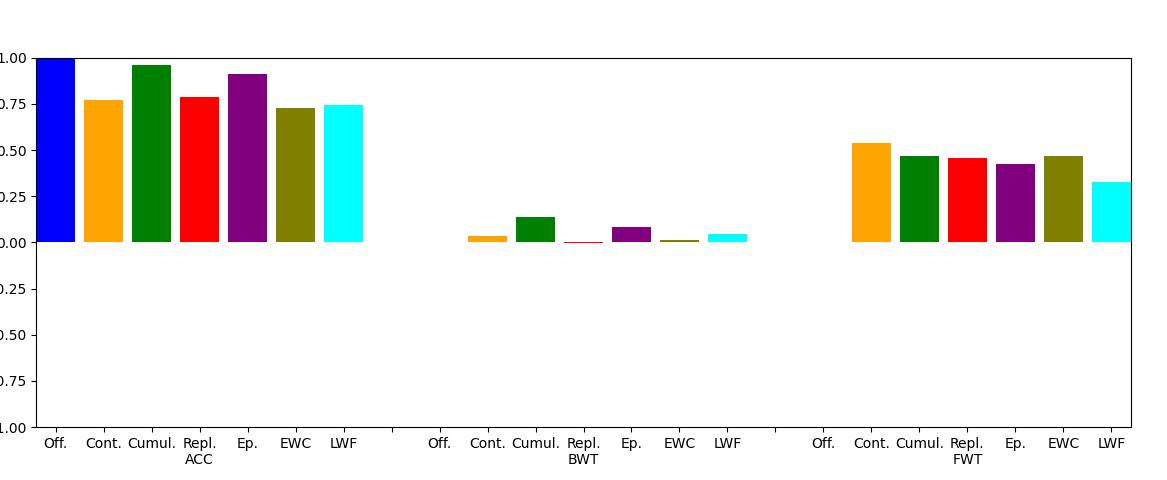
\includegraphics[width=0.95\textwidth]{img/graphs/wesad_final_metrics.png}
		\caption{Risultati WESAD}
		\label{fig:wesad_metrics_graph}
	\end{center}
\end{figure}

\paragraph{ASCERTAIN} Usando come modello due layer GRU da 24 unità, su ASCERTAIN ho ottenuto i seguenti risultati:
\begin{table}[h]
\footnotesize
    \begin{tabular}{l|c|c|c|c|c|c|c}
        \textbf{Scenario} & \textbf{Epoche} & \textbf{Tempo} & \textbf{Acc.} & \textbf{ACC} & \textbf{BWT} & \textbf{FWT} & \textbf{Memoria}\\
        \hline
         \textbf{Offline} & 3 & 29,14s & 42,78 & - & - & - & 1817,28 Mb\\
        \textbf{Continual} & 10,88$\pm$5,01 & 249,28s & 37,45$\pm$5,01 & 0,25 & -0,0168 & 0,0213 & 2154,36 Mb\\
        \textbf{Cumulative} & 9,25$\pm$6,81 & 932,56s & 39,06$\pm$4,26 & 0,2697 & 0,0064 & 0,0278 & 2297,17 Mb\\
        \textbf{Replay} & 13,25$\pm$10,03 & 402,96s & 39,48$\pm$4,37 & 0,2603 & -0,014 & 0,0485 & 2173,95 Mb\\
        \textbf{Episodic} & 12,62$\pm$7,94 & 498,24s & 38,80$\pm$4,04 & 0,2742 & 0,0048 & 0,0156 & 2231,42 Mb\\
        \textbf{EWC} & 24,14$\pm$16,94 & 810,96s & 36,08$\pm$5,66 & 0,2497 & -0,0183 & -0,0003 & 2171,62 Mb\\
        \textbf{LWF} & 21,62$\pm$10,20 & 879,68s & 35,69$\pm$5,43 & 0,2448 & 0.0327 & 0,0156 & 2103 Mb\\
    \end{tabular}
    \caption{Risultati ASCERTAIN}
    \label{tab:resascertain}
\end{table}
\begin{figure}[h]
	\begin{center}
		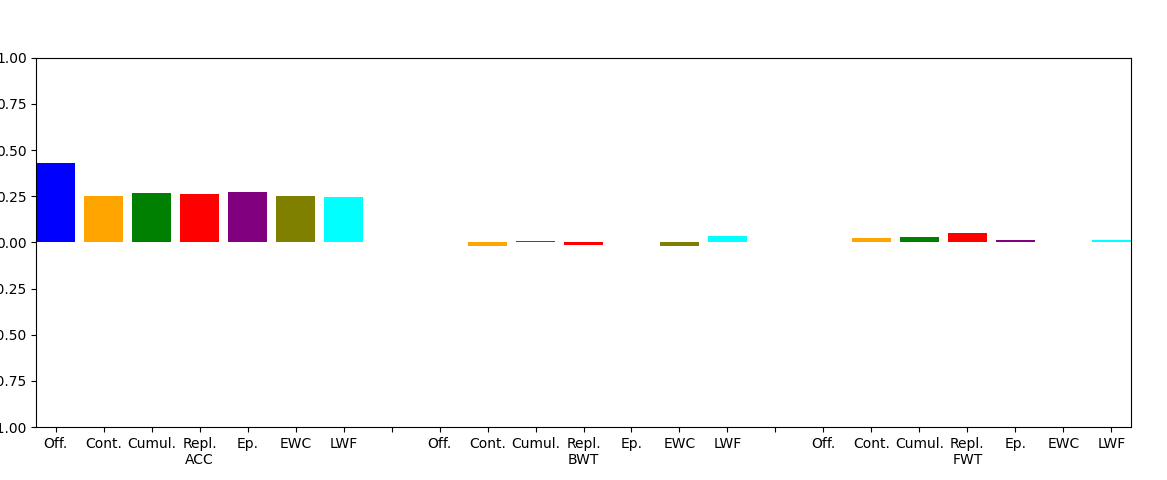
\includegraphics[width=0.95\textwidth]{img/graphs/ascertain_final_metrics.png}
		\caption{Risultati ASCERTAIN}
		\label{fig:ascertain_metrics_graph}
	\end{center}
\end{figure}
\paragraph{Custom ASCERTAIN} Usando come modello due layer GRU da 24 unità, su ASCERTAIN con i soggetti fittizi ho ottenuto i seguenti risultati:
\begin{table}[h]
\footnotesize
    \begin{tabular}{l|c|c|c|c|c|c|c}
        \textbf{Scenario} & \textbf{Epoche} & \textbf{Tempo} & \textbf{Acc.} & \textbf{ACC} & \textbf{BWT} & \textbf{FWT} & \textbf{Memoria}\\
        \hline
         \textbf{Offline} & 29 & 66,17s & 87,77 & - & - & - & 1945,91 Mb\\
        \textbf{Continual} & 7,75$\pm$5,33 & 226,24s & 87,01$\pm$0,64 & 0,2481 & -0,0241 & 0,0052 & 2143,71 Mb\\
        \textbf{Cumulative} & 7,25$\pm$8,80 & 872,8s & 87,66$\pm$0,16 & 0,2773 & 0,0032 & 0,0801 & 2273,07 Mb\\
        \textbf{Replay} & 12,125$\pm$12,94 & 299,52s & 87,13$\pm$0,75 & 0,2711 & -0,0012 & 0,306 & 2146,35 Mb\\
        \textbf{Episodic} & 5,5$\pm$3,94 & 319,76s & 82,19$\pm$3,95 & 0,339 & 0,0346 & 0,1043 & 2204,84 Mb\\
        \textbf{EWC} & 14,38$\pm$7,58 & 541,68s & 87,34$\pm$0,42 & 0,2467 & -0,0191 & 0,0845 & 2146,36 Mb\\
        \textbf{LWF} & 20,75$\pm$8,42 & 771,36s & 86,91$\pm$0,89 & 0,2495 & -0,0333 & -0,146 & 2095,93 Mb\\
    \end{tabular}
    \caption{Risultati ASCERTAIN con soggetti fittizi bilanciati}
    \label{tab:rescustonascertain}
\end{table}
\begin{figure}[h]
	\begin{center}
		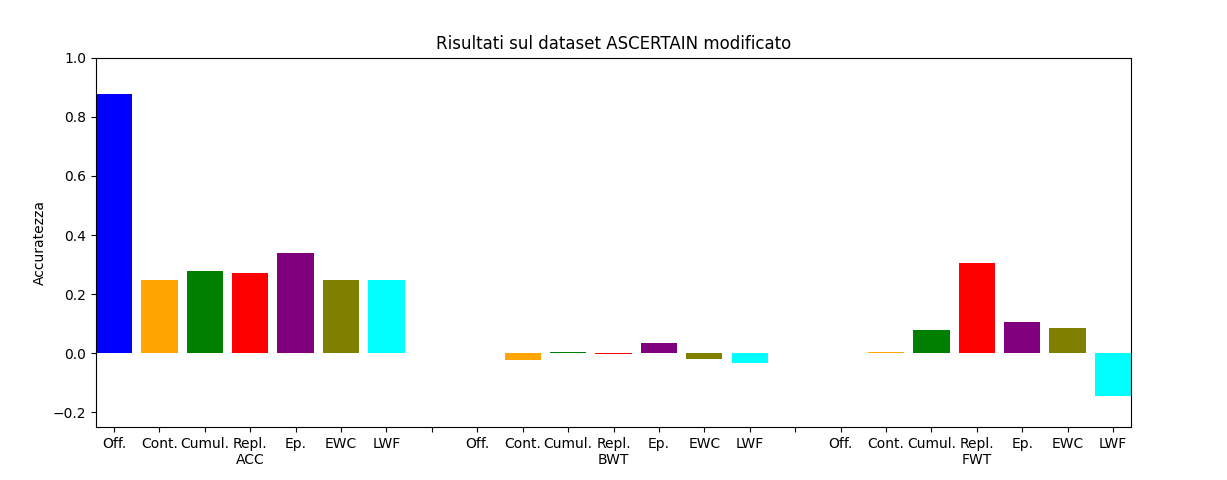
\includegraphics[width=0.95\textwidth]{img/graphs/customascertain_final_metrics.png}
		\caption{Risultati ASCERTAIN con soggetti fittizi}
		\label{fig:customascertain_metrics_graph}
	\end{center}
\end{figure}
%TODO ...scrivere